\documentclass{article}
\usepackage[utf8]{inputenc}
\usepackage[italian]{babel}
\usepackage[T1]{fontenc}
\renewcommand{\baselinestretch}{1.5}

\title{Meccanica razionale}
\author{matildetozzi}
\date{July 2020}

\usepackage{graphicx}
\graphicspath{ {./MR_images/} }
\usepackage{wrapfig}
\usepackage{natbib}
\usepackage{amsmath}
\usepackage{array}
\usepackage{geometry}
 \geometry{
 a4paper,
 total={170mm,257mm},
 left=10mm,
 right=10mm,
 top=5mm,
 bottom=5mm,
}

\begin{document}
\thispagestyle{empty}
Geometria delle masse:

\begin{tabular}{ |m{4cm}|m{7cm}|m{6cm}| } 
 \hline
 Quantità & Sistema punti & Corpo rigido esteso \\ 
 \hline
 Massa & $M = \sum_{i} m_i$ & $M = \int_{B} \rho(\underline{x}) d\underline{x}$, $\rho(\underline{x})$ densità del corpo \\ 
 \hline 
 Baricentro & $\underline{G} = \frac{\sum_{i}\underline{x}_{i}m_{i}}{M}$ somma pesata & $\underline{G} = \frac{1}{M}\int_{B}\underline{x}\rho(\underline{x})d\underline{x}$ integrale di linea (1D), superficie (2D), volume (3D)\\
 \hline
 Inerzia rispetto asse a & $I_{a} = \sum_{i} m_i r_{i}^{2}$, $r_{i}$ distanza di i dall'asse a & $I_{a} = \int_{B} r_{a}^{2}(\underline{x})\rho(\underline{x})d\underline{x}\geq 0$ \\ 
 \hline
 Prodotti di inerzia (m. centrifughi) & $I_{ab} = -\sum_{i} m_{i}a_{i}b_{i}$ & $I_{ab} = -\int_{B} {\rho(\underline{x})ab} \,da \,db$ \\
 \hline
\end{tabular}

Teorema di Huygens - Steiner:
$I_{a} = I_{a_{G}} + M d^{2}_{a-a_{G}}$
| Quantità di moto del sistema (N punti materiali): $\underline{Q}=\sum_{i=1}^{N}m_{i}\underline{v}_{i}$ oppure $\underline{Q}=M\underline{v}_{G}$ 
| Momento della quantità di moto:
$\underline{K}_{Q} = \sum_{i=1}^{N}(\underline{P}_{i}-\underline{Q})\times m_{i}\underline{v}_{i}$
SE sistema rigido:
$\underline{K}_{Q} = M (\underline{G}-\underline{Q})\times\underline{v}_{Q} + \underline{\underline{I}}_{Q}\underline{\omega}$
| Legge di distrubuzione delle velocità
$\underline{v}_{A} = \underline{v}_{B}+ \underline{\omega} \times (\underline{A}-\underline{B}) $
| I eq. card. statica
$\sum_{i} \underline{F}_{i} = \underline{0}$
| II eq. card. statica
$\sum_{i} (\underline{P}_{i} - \underline{P}) \times \underline{F}_{i} = \underline{0}$ (P polo scelto)
| Lavoro infinitesimo delle forze attive
$\delta L^{(a)} = \sum_{i} \underline{F}_{i}^{(a)} \delta \underline{P}_{i} = Q_{x_{n}} \delta \underline{x}_{n}$ (con n gdl)
| Stabilità dell'equilibrio 
$\partial_{x_{n}}U = Q_{x_{n}}$ trovare massimo potenziale e minimo pot. (eq. stabile e instabile) grazie a $\underline{\underline{H}}$
(se punti di confine, $\delta L^{(a)} (\underline{x}) \leq 0$, con $\underline{x}$ pt. di confine)
| Energia cinetica corpo rigido
$T = \frac{1}{2}M|\underline{v}_{Q}|^{2} + M \underline{v}_{Q} \cdot \underline{\omega} \times (\underline{G}-\underline{Q}) + \frac{1}{2} \underline{\underline{I}}_{Q}\underline{\omega} \cdot \underline{\omega}$ con Q punto qualsiasi (si consiglia punto fisso del sistema, punto di istantanea rotazione, oppure baricentro)
e anche 
$T = \frac{1}{2}\underline{\underline{A}}\, \underline{\Dot{q}}\cdot \underline{\Dot{q}}$ con $\underline{\underline{A}} = \begin{bmatrix}
\frac{\partial^2 T}{\partial \Dot{q}_1^2} & \frac{\partial^2 T}{\partial \Dot{q}_1 \partial \Dot{q}_2}\\
\frac{\partial^2 T}{\partial \Dot{q}_1 \partial \Dot{q}_2} & \frac{\partial^2 T}{\partial \Dot{q}_2^2} 
\end{bmatrix}$ (esempio 2D) matrice di massa (simmetrica) e $\underline{q}$ coordinate lagrangiane
| Equazione dei piccoli moti
$\underline{\underline{A}}(\underline{q}_{e})\underline{\ddot{\eta}}-\underline{\underline{H}}(\underline{q}_{e})\underline{\eta}=\underline{0}$ con $\underline{q}_{e}$ punto di equilibrio e $\underline{\eta}=\underline{q}-\underline{q}_e$ piccole oscillazioni
| Equazioni di Lagrange 
$\frac{d}{dt}\frac{\partial T}{\partial \Dot{q}} - \frac{\partial T}{\partial q} = Q_p^{(a)}$
| I eq. card. dinamica
$m_{s}\underline{a}_{G_{s}} = \underline{R}^{(e)} = \sum_{i}\underline{F}_{i} + \sum_{j}\underline{\Phi}_{j}$
| II eq. card. dinamica
$\underline{\Dot{K}}_{\Omega} + \underline{\Dot{\Omega}} \times \underline{Q} = \underline{M}_{\Omega}^{(e)} = \underline{M}_{\Omega}^{(e,a)} + \underline{M}_{\Omega}^{(e,v)}$
| Lagrangiana
$L = T + U$
| Momento cinetico rispetto a $x$ =
$\frac{\partial L}{\partial x}$
\begin{wraptable}{r}{6cm}
\begin{tabular}{|c|c|}
\hline
Momenti di inerzia & \\
\hline
Triangolo isoscele & $I_G = \frac{ml^2}{9}$ \\
Asta & $I_{G} = \frac{ML^{2}}{12}$ \\
Disco & $I_{G} = \frac{MR^2}{2}$ \\
Anello & $I_G = mR^2$ \\
Lastra & $I_G = \frac{m(a^{2} + b^{2})}{12}$ \\
\hline
\end{tabular}
\end{wraptable}
\begin{wraptable}{l}{6cm}
\begin{tabular}{|c|c|}
\hline
Capire max e min & \\
\hline
Det. pos. e traccia pos. & minimo \\
Det. pos. e traccia neg. & massimo \\
\hline
\end{tabular}
\end{wraptable}
$\cos{\arcsin{\lambda}} = \sqrt{1-\lambda^2}$ \,
$\sin{\arccos{\lambda}} = \sqrt{1-\lambda^2}$ \,
$\int \cos \theta \sin \theta \, d \theta = \frac{\sin^2 \theta}{2}$ \,
$\int \sin^2 \theta \, d \theta = \frac{\theta}{2} - \frac{\cos \theta \sin \theta}{2}$ \,
$\int \cos^2 \theta \, d \theta = \frac{\theta}{2} + \frac{\cos \theta \sin \theta}{2}$ \,
$(\tan x)' = \frac{1}{\cos^2 x}$

$\cos \theta = \lambda \xrightarrow{} \theta_2 = 2\pi - \arccos{\lambda}$ \,
$\sin \theta = \lambda \xrightarrow{} \theta_2 = \pi - \arcsin{\lambda}$
\begin{figure}[!]
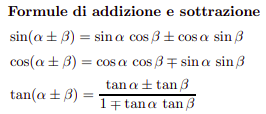
\includegraphics[width=5cm]{addizione.png}
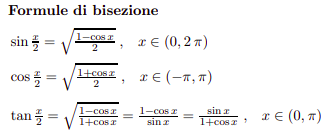
\includegraphics[width=7cm]{bisezione.png}
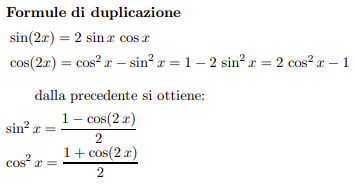
\includegraphics[width=6cm]{duplicazione.png}
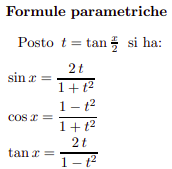
\includegraphics[width=4cm]{parametriche.png}
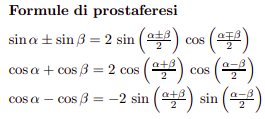
\includegraphics[width=5cm]{prostaferesi.png}
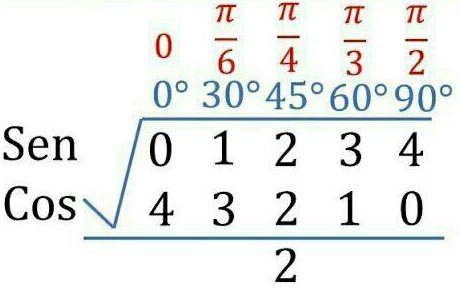
\includegraphics[width=3cm]{valori.jpg}
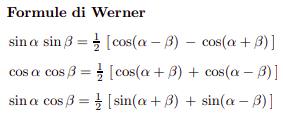
\includegraphics[width=5cm]{werner.png}
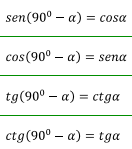
\includegraphics[width=3cm]{ass1.png}
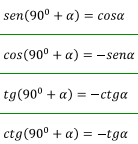
\includegraphics[width=3cm]{ass2.png}
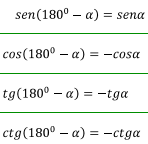
\includegraphics[width=3cm]{ass3.png}
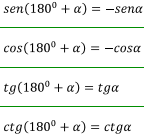
\includegraphics[width=3cm]{ass4.png}
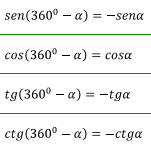
\includegraphics[width=3cm]{ass5.png}
\end{figure}
\end{document}